\documentclass[a4paper,11pt,oneside]{article}
\usepackage[T1]{fontenc}
\usepackage[utf8x]{inputenc}
\usepackage{lmodern,textcomp}
\usepackage[document]{ragged2e}
\usepackage{longtable}
\usepackage[USenglish]{babel}
\usepackage[dvipsnames]{xcolor}

\usepackage[calc,useregional]{datetime2}
\usepackage{datenumber}
\usepackage{calc}
\newcounter{datetoday}
\newcounter{diffyears}
\newcounter{diffmonths}
\newcounter{diffdays}
\newcommand{\difftoday}[3]{%
      \setmydatenumber{datetoday}{\the\year}{\the\month}{\the\day}%
      \setmydatenumber{diffdays}{#1}{#2}{#3}%
      \addtocounter{diffdays}{-\thedatetoday}%
      \ifnum\value{diffdays}<0
        \setcounter{diffdays}{-\value{diffdays}}%
      \fi
      \setcounter{diffyears}{\value{diffdays}/365}%
      \setcounter{diffdays}{\value{diffdays}-365*\value{diffyears}}%
      \setcounter{diffmonths}{\value{diffdays}/30}%
      \setcounter{diffdays}{\value{diffdays}-30*\value{diffmonths}}%
      \ifnum\value{diffyears}=0
      \else
        \ifnum\value{diffyears}>1
            \thediffyears\space yrs
        \else
            \thediffyears\space yr
        \fi
      \fi
      \ifnum\value{diffmonths}=0
        1 mo
      \else
        \ifnum\value{diffmonths}>1
            \thediffmonths\space mos
        \else
            \thediffmonths\space mo
        \fi
      \fi
}

\newcommand{\fakesection}[1]{
  \par\refstepcounter{section}
  \sectionmark{#1}
  \addcontentsline{toc}{section}{#1}
}

\usepackage{advdate}
\usepackage{setspace}
\usepackage{hyperref}
\usepackage{url}
\hypersetup{colorlinks=true,linkcolor=RoyalBlue,urlcolor=RoyalBlue,citecolor=RoyalBlue,anchorcolor=RoyalBlue}
\urlstyle{same}
\usepackage{graphicx}
\usepackage[export]{adjustbox}
\usepackage{colortbl}

\usepackage[left=2cm,right=2cm,bottom=2cm,top=1.5cm,foot=0.5cm]{geometry}

\usepackage{lastpage}
\usepackage{fancyhdr}
\fancypagestyle{plain}{\fancyhead{}\renewcommand{\headrule}{}}
\pagestyle{plain}
\fancyhead{}
\renewcommand{\headrulewidth}{0pt}
\fancyfoot{}
\fancyfoot[L]{\small {\color{gray}Stéphane Ghozzi $\cdot$ Curriculum vitae as of \today}} 
\fancyfoot[R]{\small {\color{gray}page\ \thepage\ of \pageref*{LastPage}}}
\pagenumbering{arabic}

\setcounter{secnumdepth}{0}
\usepackage{tocloft}
\renewcommand{\cftsecleader}{\cftdotfill{\cftsecdotsep}}
\renewcommand\cftsecdotsep{\cftdot}

\hyphenation{di-sease tra-vel-ling ana-ly-ses rea-lize vi-sua-li-za-tion a-na-ly-zing}

\usepackage{cite}

\begin{document}
\selectlanguage{USenglish}

\noindent\begin{minipage}{0.7\linewidth}
   \LARGE
   \noindent\textbf{Stéphane Ghozzi}

   \normalsize
   \vspace{1.5em}
   \noindent Researcher interested in supporting public health preparedness and response through automated analyses and visualizations: application and evaluation of machine-learning approaches, development and deployment of interactive dashboards. Moved from fundamental theoretical physics to biophysics and now infectious-disease epidemiology. Loves assembling interdisciplinary teams, comfortable as independent analyst and developer. 
\end{minipage}
\begin{minipage}{0.3\linewidth}
   \begin{center}
      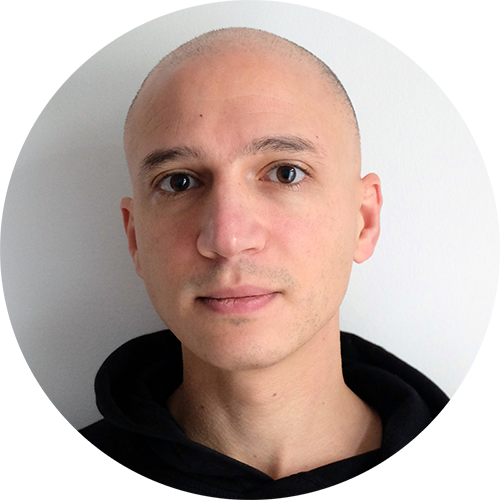
\includegraphics[width=0.55\textwidth,right]{GHOZZI-Stephane-portrait-2020-cropped-circle-nobackground-lr.png}
   \end{center}
\end{minipage} 

\vspace{1em}

\href{https://orcid.org/0000-0002-3911-9573}{orcid.org/0000-0002-3911-9573} $\cdot$ \href{https://gitlab.com/stephaneghozzi}{gitlab.com/stephaneghozzi} $\cdot$
\href{https://twitter.com/stephaneghozzi}{twitter.com/stephaneghozzi} $\cdot$\\ \href{https://www.linkedin.com/in/stephaneghozzi}{linkedin.com/in/stephaneghozzi} $\cdot$ \href{https://scholar.google.com/citations?user=uGVLwREAAAAJ}{scholar.google.com/citations?user=uGVLwREAAAAJ} $\cdot$ \\
\href{https://www.researchgate.net/profile/Stephane\_Ghozzi}{researchgate.net/profile/Stephane\_Ghozzi}

\vspace{1em}

\noindent {\color{gray}\hrule} 

\vspace{1em}

\noindent \begin{longtable}{@{}p{3.1cm}@{}@{}p{13.9cm}@{}}
   \Large{Experience} & \\
   & \\
   \textbf{Research} & \textbf{Helmholtz-Zentrum für Infektionsforschung (HZI)} \\
   \textbf{associate} & {\color{gray}\DTMdisplaydate{2020}{6}{1}{-1} -- present $\cdot$ \difftoday{2020}{6}{1}} \\ 
   & {\color{gray} Brunswick (Braunschweig), Germany} \\
   & \href{https://www.helmholtz-hzi.de/en/research/research-topics/bacterial-and-viral-pathogens/epidemiology/our-research/}{helmholtz-hzi.de/en/research/research-topics/bacterial-and-viral-pathogens/epidemiology/our-research/} $\cdot$ \href{https://sormas.org}{sormas.org} \\ 
   & Senior scientist, statistical methods and tools for public health, in the Epidemiology department (Krause group). \\
   & \\
   & \begin{tabular}[t]{@{}!{\color{gray}\vrule}p{0.2cm}@{}p{13.3cm}@{}}
      & Surveillance Outbreak Response Management and Analysis System (SORMAS): Automated support for decision making by SORMAS users. Strategies to bring computations to data so as to allow for advanced analytics without compromising data privacy. \\
      & \\
      & Effect of climate change on infectious disease spread: Statistical modelling of the impact of short and long-term environmental and demographic changes on Lyme disease spread in Germany. \\
      & \\
      & Machine learning for multiplex serology.\\
      & \\
      & Management and organization: \\
      & $\cdot$ contact person for topics of automated analyses and processes ; \\
      & $\cdot$ student support ; \\
      & $\cdot$ writing of grant applications. \\
   \end{tabular} \\      
   & \\
   & \\   
   & \textbf{Robert-Koch Institut (RKI)} \\
   & {\color{gray}\DTMdisplaydate{2016}{4}{15}{-1} -- \DTMdisplaydate{2020}{5}{31}{-1} $\cdot$ 4 yrs 2 mos}\\ 
   & {\color{gray}Berlin, Germany}\\
   & \href{https://www.rki.de/signale-project}{rki.de/signale-project} \\
   & Machine learning, informatics, statistics and visualizations, Signale team, Department of Infectious-Disease Epidemiology. \\
   & \\
   & \begin{tabular}[t]{@{}!{\color{gray}\vrule}p{0.2cm}@{}p{13.3cm}@{}}
      & Research and development: \\
      & $\cdot$ development of outbreak-detection algorithms and modelling of infection dynamics; \\
      & $\cdot$ performance evaluation and parameter optimization of the algorithms; \\
      & $\cdot$ natural language processing of online articles to support international infectious-disease surveillance; \\
      & $\cdot$ interactive visualizations of the results and other data for public-health professionals. \\
      & \\
      & Management and organization: \\
      & $\cdot$ speaker for the team (four data scientists, two web developers, an average of two students); \\
      & $\cdot$ coordination of the international Topic Group Outbreaks under the Focus Group AI for Health of ITU and WHO: \href{https://www.itu.int/en/ITU-T/focusgroups/ai4h/Pages/tg.aspx}{itu.int/en/ITU-T/focusgroups/ai4h/Pages/tg.aspx} \\
      & $\cdot$ supervision of master theses; \\
      & $\cdot$ organization of workshops and hackathons; \\
      & $\cdot$ writing of grant applications. \\
   \end{tabular} \\
   & \\
   & \\
   & \textbf{World Health Organization (WHO)} \\
   & {\color{gray}\DTMdisplaydate{2019}{5}{1}{-1} -- \DTMdisplaydate{2019}{10}{31}{-1} $\cdot$ 6 mos} \\ 
   & {\color{gray}Geneva, Switzerland} \\
   & \href{https://www.who.int/eios}{who.int/eios} $\cdot$ \href{https://www.who.int/emergencies/outbreak-toolkit}{who.int/emergencies/outbreak-toolkit} \\
   & Machine learning and web-application development for epidemic intelligence and investigation of outbreaks of unknown origins. \\
   & \\
   & \begin{tabular}[t]{@{}!{\color{gray}\vrule}p{0.2cm}@{}p{13.3cm}@{}}
      & In the Detection, Verification and Risk Assessment (DVA) and the Health Operations Monitoring and Data Collection (MDC) units of the Health Emergency Information and Risk Assessment (HIM) department within the WHO Health Emergencies (WHE) program of WHO. \\
   \end{tabular} \\
   & \\
   & \\
   \textbf{Visual artist} & \textbf{self employed} \\
   & {\color{gray}\DTMdisplaydate{2012}{3}{1}{-1} -- \DTMdisplaydate{2016}{4}{14}{-1} $\cdot$ 4 yrs 1 mo} \\ 
   & {\color{gray}Berlin, Germany} \\
   & \href{http://www.stephaneghozzi.com}{stephaneghozzi.com} \\
   & Drawing, generative animation, photography, video, computer animation. \\
   & \\   
   & \begin{tabular}[t]{@{}!{\color{gray}\vrule}p{0.2cm}@{}p{13.3cm}@{}}   
      & Selected projects and collaborations: \\
      & $\cdot$ 2014: videos exhibited during the \textit{backup} festival, E-Werk, Weimar; \\
      & $\cdot$ 2005: twelve illustrations for \textit{Trace.project}, a compilation album of original electronic music; \\
      & $\cdot$ 2005: videography for the dance piece \textit{Entre-Deux} by Mirjam Fruttiger, Paris and Rome (including one-week invitation at the Villa Médicis); \\
      & $\cdot$ 2004: videography on the documentary \textit{Manchay Tiempo} by Florence Blum and María Pía Medina-Luna (four-weeks filming in Peru); \\
      & $\cdot$ 2002: drawings and photographs published in the magazine \textit{R de réel}. \\
   \end{tabular} \\   
   & \\
   & \\
   \textbf{Postdoctoral} & \textbf{Institut für Theoretische Physik (THP), Universität zu Köln}\\
   \textbf{researcher} & {\color{gray}\DTMdisplaydate{2010}{3}{1}{-1} -- \DTMdisplaydate{2012}{2}{29}{-1} $\cdot$ 2 yrs}\\
   & {\color{gray}Cologne, Germany} \\
   & \url{www.thp.uni-koeln.de/~lassig} \\
   & Statistical and mechanical models of biological evolution, in the Lässig group. \\
   & \\
   & \begin{tabular}[t]{@{}!{\color{gray}\vrule}p{0.2cm}@{}p{13.3cm}@{}}
      & Mathematical model and analysis of bacterial growth and gene expression, interpretation of experimental results. \\
      & \\
      & Signatures of selection in DNA sequences and comparison with population genetics models: \\
      & $\cdot$ long-term influenza evolution; \\
      & $\cdot$ transcription-binding-site motifs in yeast. \\
      & \\
      & Co-evolution signatures in protein sequences. \\
   \end{tabular} \\   
   & \\   
   & \\   
   \textbf{Teaching} & \textbf{Universität zu Köln} \\
   \textbf{assistant} & {\color{gray}\DTMdisplaydate{2010}{9}{1}{-1} -- \DTMdisplaydate{2012}{1}{30}{-1} $\cdot$ 1 yr 5 mos} \\
   & {\color{gray}Cologne, Germany} \\   
   & Mathematics and statistical physics for Bachelor students.\\
   & \\
   & \textbf{UPMC Sorbonne Universités} \\
   & {\color{gray}\DTMdisplaydate{2005}{10}{1}{-1} -- \DTMdisplaydate{2009}{8}{31}{-1} $\cdot$ 3 yrs 11 mos} \\
   & {\color{gray}Paris, France} \\
   & Thermodynamics, optics and waves, mathematical methods for Bachelor students. \\
   & \\   
   & \\   
   \textbf{Doctoral} & \textbf{Laboratoire de Physique Statistique (LPS), École normale supérieure} \\
   \textbf{researcher} & {\color{gray}\DTMdisplaydate{2005}{9}{1}{-1} -- \DTMdisplaydate{2009}{12}{31}{-1} $\cdot$ 4 yrs 4 mos} \\
   & {\color{gray}Paris, France} \\
   & \href{http://www.labos.upmc.fr/ljp/?article7}{www.labos.upmc.fr/ljp/?article7} $\cdot$ \href{http://www.lps.ens.fr/?lang=en}{www.lps.ens.fr} \\
   & Theoretical and experimental biophysics, in the Chatenay group: Dynamics of gene regulatory networks. \\
   & \\
   & \begin{tabular}[t]{@{}!{\color{gray}\vrule}p{0.2cm}@{}p{13.3cm}@{}}
      & Won a 60 k€ grant to fund the experimental project (over 3 years, used to buy apparatus and consumables): program ``Interface physique, biologie et chimie : soutien à la prise de risque 2007-2009'' of the CNRS. \\
      & \\
      & Time series of gene expression levels, via fluorescent microscopy, of the lysis-lysogeny decision network of the bacteriophage Lambda: \\
      & $\cdot$ molecular biology (extraction of viral genes, insertion of genes coding for fluorescent protein, modification of bacterial genomes); \\
      & $\cdot$ microbiology (bacterial and viral cultures); \\
      & $\cdot$ automation and fluorescent microscopy; \\
      & $\cdot$ image analysis. \\   
      & \\
      & Mathematical analysis of noise statistics of bacterial gene expression. \\
      & \\
      & Computer simulations of the dynamics and evolution of gene regulatory networks. \\ 
   \end{tabular} \\
   & \\
   & \\   
   \textbf{Volunteering} & \textbf{Celsius} \\
   \textbf{Founding} & {\color{gray}\DTMdisplaydate{2007}{8}{1}{-1} -- \DTMdisplaydate{2009}{8}{31}{-1} $\cdot$ 2 yrs 1 mo} \\
   \textbf{member} & {\color{gray}Paris, France} \\
   & Celsius was a think tank with the goal of developing the European project. \\
   & \\   
   & \begin{tabular}[t]{@{}!{\color{gray}\vrule}p{0.2cm}@{}p{13.3cm}@{}}
      & $\cdot$ Elaboration of background documents on technical themes; \\
      & $\cdot$ preparation, organization of, and follow-up on, two-days meetings in Madrid, Brussels, and Paris, each with more than 30 participants; \\
      & $\cdot$ development of publication strategies, print and online. \\
   \end{tabular} \\
   & \\
   & \\   
   \textbf{Internships} & \textbf{Laboratoire de l'Accélérateur Linéaire (LAL), Université Paris-Sud} \\
   & {\color{gray}\DTMdisplaydate{2005}{2}{1}{-1} -- \DTMdisplaydate{2005}{3}{31}{-1} $\cdot$ 2 mos} \\
   & {\color{gray}Orsay, France} \\
   & Theoretical particle physics, in the Davier group: Computation of fundamental physical quantities for high energy physics from particle collision experiments data. \\
   & \\
   & \textbf{Deutsches Elektronen-Synchrotron (DESY), Humboldt-Universität zu Berlin} \\
   & {\color{gray}\DTMdisplaydate{2003}{1}{17}{-1} -- \DTMdisplaydate{2003}{8}{31}{-1} $\cdot$ 7 mos} \\
   & {\color{gray}Zeuthen, Germany} \\
   & Theoretical particle physics, in the Jegerlehner group: Analysis of experimental data with ad hoc and first-principle mathematical models of elementary particles. \\
   & \\
   & \textbf{Laboratoire Kastler Brossel (LKB), École normale supérieure} \\
   & {\color{gray}\DTMdisplaydate{2002}{6}{1}{-1} -- \DTMdisplaydate{2002}{8}{31}{-1} $\cdot$ 3 mos} \\
   & {\color{gray}Paris, France} \\   
   & Experimental quantum physics, in the Grynberg group: Construction of an optical atom trap. \\
\end{longtable}

\vspace{1em}

\noindent {\color{gray}\hrule} 
   
\vspace{1em}
   
\noindent \begin{longtable}{@{}p{3.1cm}@{}@{}p{13.9cm}@{}}
   \Large{Education} & \\
   & \\
   \textbf{Certifications} & \textbf{Coursera}\\
   & {\color{gray}\DTMdisplaydate{2016}{1}{1}{-1} -- \DTMdisplaydate{2016}{3}{31}{-1} $\cdot$ 3 mos} \\
   & Practical Predictive Analytics: Models and Methods \\
   & Machine Learning \\
   & Data Manipulation at Scale: Systems and Algorithms \\
   & \\
   & \\   
   \textbf{Ph.D.} & \textbf{École normale supérieure}\\
   & {\color{gray}\DTMdisplaydate{2005}{9}{1}{-1} -- \DTMdisplaydate{2009}{12}{31}{-1} $\cdot$ 4 yrs 4 mos} \\
   & {\color{gray}Paris, France} \\
   & Theoretical and experimental biophysics: Dynamics of gene regulatory networks. See ``Experience'' above for details. \\
   & \\
   & \\   
   \textbf{B.Sc. \&} & \textbf{École normale supérieure} \\
   \textbf{M.Sc.} & {\color{gray}\DTMdisplaydate{2001}{9}{1}{-1} -- \DTMdisplaydate{2005}{8}{31}{-1} $\cdot$ 4 yrs} \\
   & {\color{gray}Paris, France} \\
   & Theoretical and mathematical physics: specialization in particle physics and statistical physics. \\
   & \\
   & \begin{tabular}[t]{@{}!{\color{gray}\vrule}p{0.2cm}@{}p{13.3cm}@{}}   
      & Competitive fellowship. \\
      & \\
      & Activities and societies: President of the Photography and Video-Making student associations in 2002 and 2003: \\
      & $\cdot$ presenting, defending, and managing budgets; \\
      & $\cdot$ initiation and support for members. \\
   \end{tabular} \\   
   & \\
   & \\   
   \textbf{M.A.} & \textbf{École nationale supérieure des arts décoratifs} \\
   & {\color{gray}\DTMdisplaydate{2003}{9}{1}{-1} -- \DTMdisplaydate{2004}{8}{31}{-1} $\cdot$ 1 yr} \\
   & {\color{gray}Paris, France} \\
   & CGI, 3d animation, post-production.
\end{longtable}

\vspace{1em}

\noindent {\color{gray}\hrule} 
   
\vspace{1em}
   
\noindent \begin{longtable}{@{}p{3.1cm}@{}@{}p{13.9cm}@{}}
   \Large{Skills} & \\
   & \\
   \textbf{Programming} & R, Python, LaTeX, Mathematica, Matlab, Processing (Java), SQL, Perl, C++, Shell \\
   & \\   
   \textbf{Tools} & Git, Jira, Confluence, Team Foundation Server (agile management: Scrum, Kanban), SQL Server Management Studio, Photoshop, Illustrator, After Effects, Microsoft Office, 3ds Max, Blender \\
   & \\   
   \textbf{Languages} & French (native) \\
   & German (professional) \\
   & English (professional) \\
   & Japanese (basics)
\end{longtable}

\vspace{1em}

\noindent {\color{gray}\hrule} 
   
\vspace{2em}
   
\noindent \Large{Publications}

\vspace{0.5em}

\normalsize
\nocite{*}
\begingroup
\renewcommand{\section}[2]{}
\bibliographystyle{./IEEEtran.bst}
\bibliography{publications_ghozzi}
\endgroup

\end{document}